\thechapter{Experimental results} 

\begin{wrapfigure}{r}{0.5\textwidth}
\centering
\begin{subfigure}[b]{0.28\textwidth}
        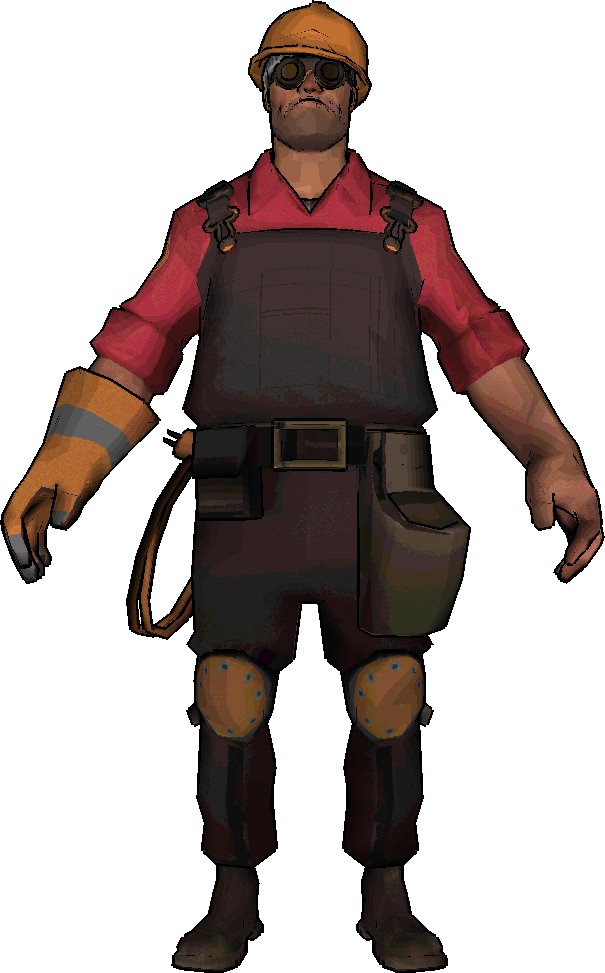
\includegraphics[width=\textwidth]{img/Textures/TextureLightingCelShade.png}
\end{subfigure}
\caption{Cel Shaded Texture Final}
 \label{fig:TextureLightingCelShade}
\end{wrapfigure} 

Our system was able to produce the best results using models with higher vertex counts and smooth curves like the skull, while the engineer was more problematic, but increasing the vertex count also significantly increased the time to produce the render. Many aspects needed to be customized to particular models to get optimal results.

When our simple Cel Shading algorithm is applied to some textures the colours output need correction especially at lower levels as in \ref{fig:CelShadeTexture4}, but combined with cel shaded lighting using more levels for the texture the desired effect can be produced \ref{fig:CelShadeTexture4}. 

%\begin{wrapfigure}{r}{0.5\textwidth}
\begin{figure}[h]
\centering
\begin{subfigure}[b]{0.18\textwidth}
        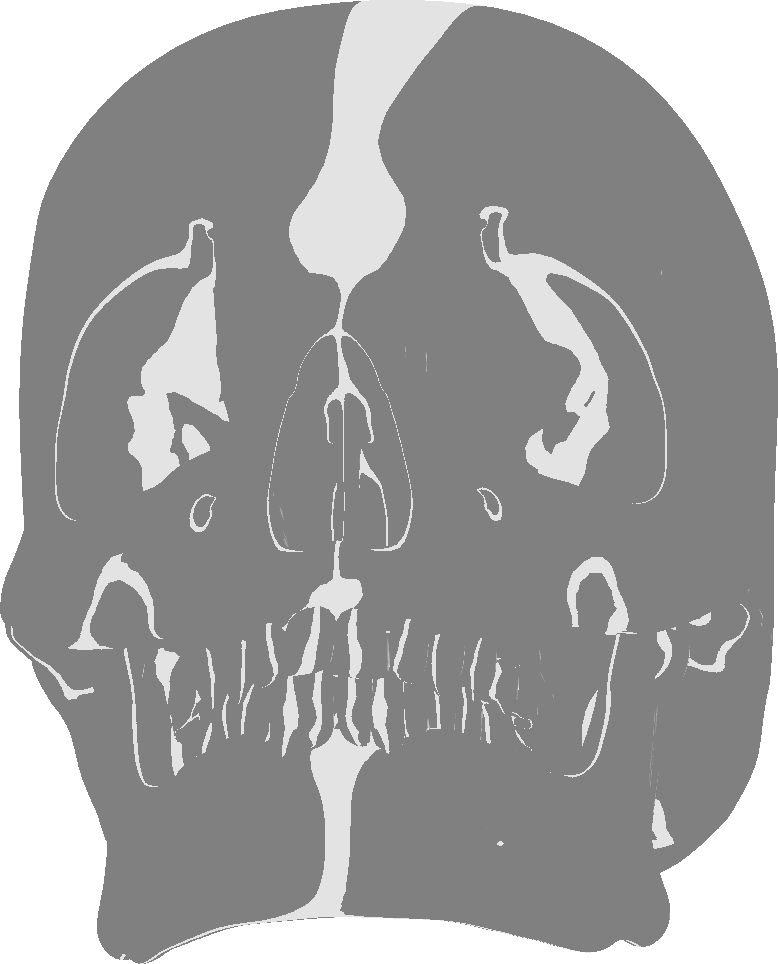
\includegraphics[width=\textwidth]{img/Lighting/Directional.png}
        \caption{Directional}
        \label{fig:LightingPosDir}
\end{subfigure}
    ~
    \begin{subfigure}[b]{0.18\textwidth}
        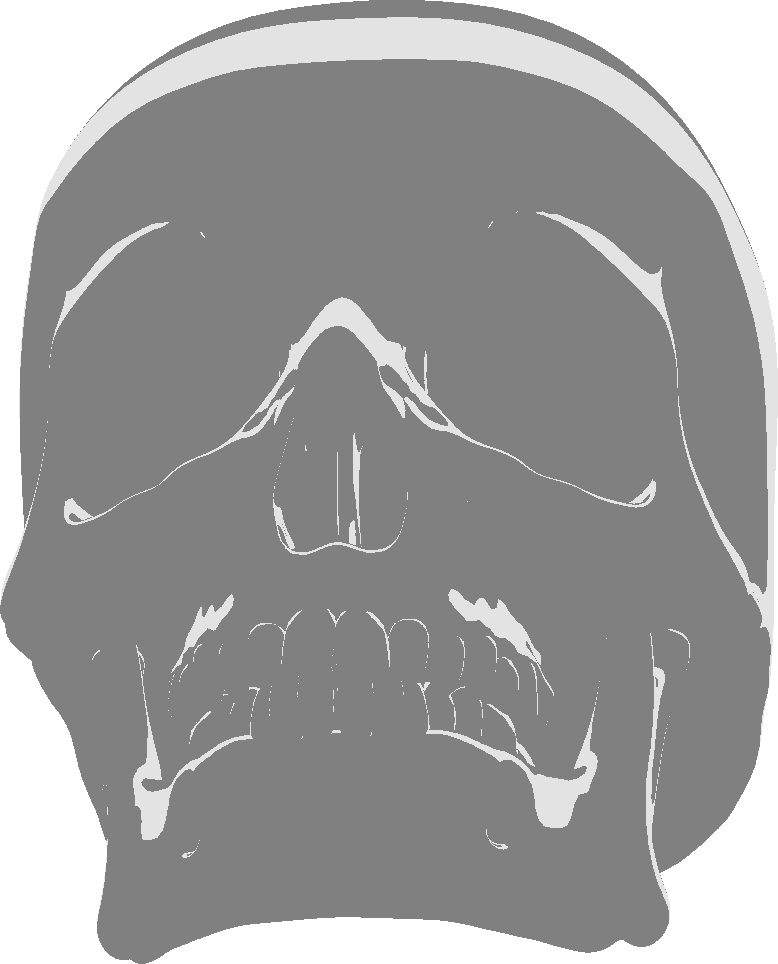
\includegraphics[width=\textwidth]{img/Lighting/Point.png}
        \caption{Point}
        \label{fig:LightingPosPos}
    \end{subfigure}
\caption{Rim Lighting and Light Position}
 \label{fig:LightingPosRim}
 \end{figure}
%\end{wrapfigure} 

Positioning of the light for optimally rending the lighting is highly dependant on the model, and the area of the model that is being viewed. Depending on the positioning of the lighting the effect can vary greatly, demonstrated in \ref{fig:LightingPosRim} where the rim lighting on the model appears dramatically different depending on the distance away it is.

As for adding in our contours and suggestive contours. We have cycled through three methods.

Our first implementation was only able to handle contours and was done using OpenGLs built- in PolygonMode system. More specifically, it was done by re-rendering the model in GL_Line mode. Before offsetting in the Z axis relative to the camera. Theoretically making it so that the only part visible would be the lines outlining the model.

\begin{figure}[h]
    \centering
    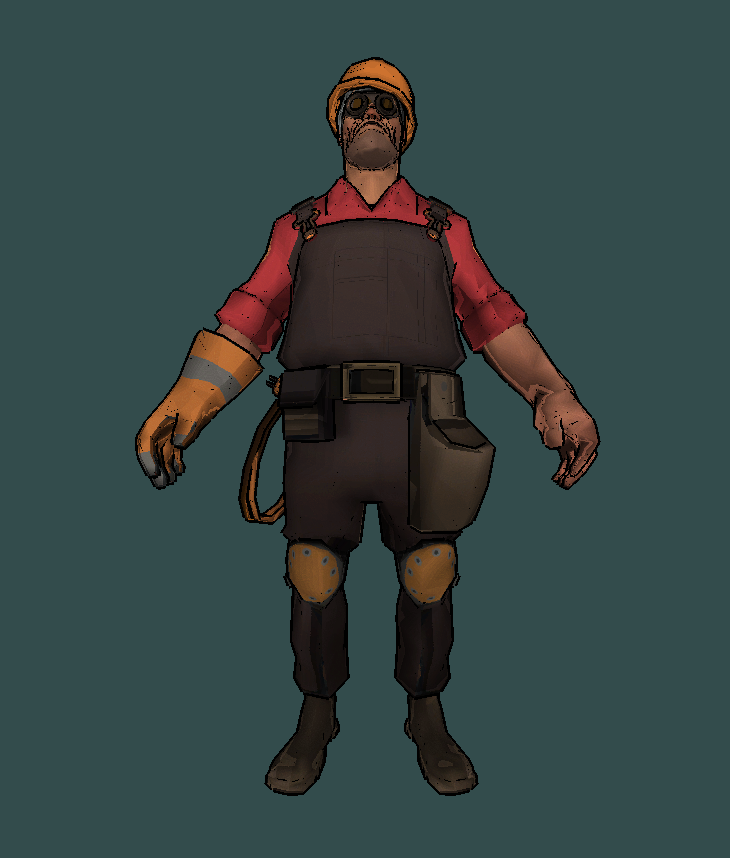
\includegraphics[width=0.5\textwidth]{img/ModelB.png}
    \caption{An overview of stages in the rendering step}
    \label{fig-render-overview}
\end{figure}

The problem with this is implementation, next to its simplicity, is that it produces a lot of artifacts. With this problem being most pronounced around the face of the model, which has the highest density of polygons. But they can be seen through the model. Flickering in and out of existence as the model is rotated.

\begin{figure}[h]
    \centering
    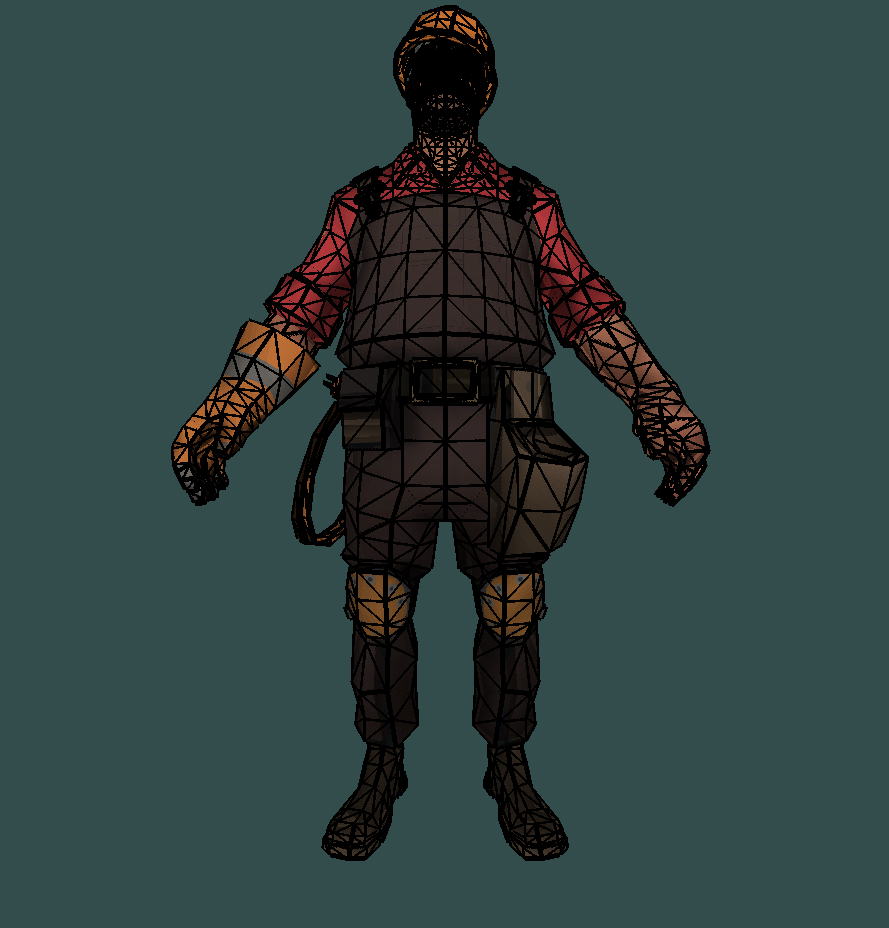
\includegraphics[width=0.5\textwidth]{img/ModelA.png}
    \caption{An overview of stages in the rendering step}
    \label{fig-render-overview}
\end{figure}

\begin{figure}[h]
    \centering
    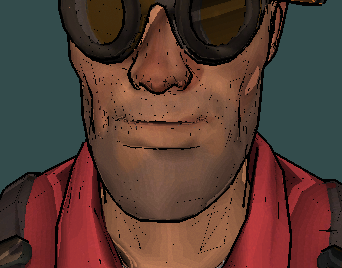
\includegraphics[width=0.5\textwidth]{img/ModelC.png}
    \caption{An overview of stages in the rendering step}
    \label{fig-render-overview}
\end{figure}

Seeing that this was not going to work, we then moved onto our second implementation using the stencil buffer. For contours, we set the stencil buffer to store the position of any pixel that was drawn before rendering the model to the screen. Before disabling writing to the buffer and inverting its data. Making it so that only areas outside that in which the model was drawn could be rendered to. Before once more rending the outline of the model.

While this was happening, suggestive contours would be calculated inside of the shaders and stored in a matrix, to be passed into the stencil buffer for a third and final pass. But it was as we were going over this that we realized that since we were already doing calculations inside of the fragment shader, it would be easier to manually set the color of the fragment to be black.

\begin{figure}[h]
    \centering
    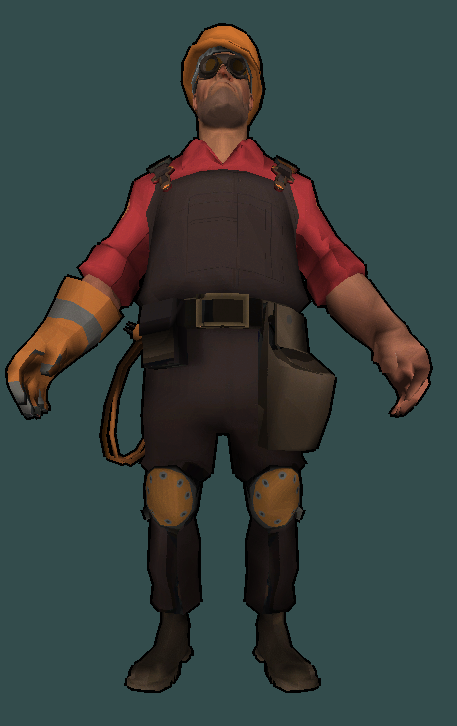
\includegraphics[width=0.5\textwidth]{img/ModelD.png}
    \caption{An overview of stages in the rendering step}
    \label{fig-render-overview}
\end{figure}

This leads into implementation three. For this implementation, we realized that it would be better to instead do all the work inside of the shaders. As most of the calculations would need to be done inside of them anyways. And by doing it this way, we would be able to generate the Contours in a single pass, instead of needing 3. While also being able to handle both Contours and Suggestive Contours in a near identical way to Contours.

For the actual implementation, we used the dot product of the normal vector of each face and the view angle. With any result of zero being a contour. While any none zero none negative result being compared to its sourdning faces. With any faces found to be significantly lower to be registerd as a Sujestive Contour. With Contours and Sujestive Contours being set to render as black once they reach the Fragment Shader.